\section{类型转换}
C++提供了丰富的基本类型,包括各种整型、浮点型、字符型和布尔型等\footnote{这里所列举的都属于算术类型。除此之外,基本类型中还有 \lstinline@void@ 和 \lstinline@nullptr_t@ 类型,但这里不讲。}。它们用途各异,表示范围也有差别。类型区分明确有很多好处,其中一点就是,许多运算符可以在操作数类型不同的情况下,表示不同的含义,得到不同的结果。将来我们会学习函数重载和运算符重载,这种方法大大增加了代码的可扩展性,并让我们可以通过自定义重载的方法针对不同类型实现多种多样的功能。前文提过,\lstinline@<<@ 在左操作数为 \lstinline@ostream@ 类时,实现输出功能;而在左操作数为整型时,定现左移位计算功能,这就是对类型多样性意义的最佳诠释。\par
但是,不同类型之间的隔阂也让人望而却步。假设我要输入两个整数并求它们的商和模值,而我们这么写代码:
\begin{lstlisting}
    int a, b; //定义两个int型变量,无须初始化
    cin >> a >> b; //输入a和b的值
    cout << a / b << endl << a % b; //输出a/b和a%b
\end{lstlisting}
那么就会出现经典问题,整型除法的返回值自动截尾,我们得到的是不精确的结果。那么如果我们把代码改成这样呢?
\begin{lstlisting}
    double a, b; //定义两个double型变量,这样double除法得到的结果就精确了
    cin >> a >> b; //输入a和b的值
    cout << a / b << endl << a % b; //输出a/b和a%b
//error: invalid operands of types 'double' and 'double'
//to binary 'operator%'
\end{lstlisting}
这样代码就会报错,因为``用 \lstinline@double@ 型数据与 \lstinline@double@ 型数据相取模是不允许的''。\par
类型限制太死板,难免就会在这种需要灵活性的地方出现问题,而C++解决这个问题的方式就是\textbf{类型转换(Type cast/Type conversion)}。\par
\subsection*{隐式类型转换}
我们知道 \lstinline@'0'@ 的ASCII码值是 \lstinline@48@,但是它是 \lstinline@char@ 型,而C++中的 \lstinline@cout<<@ 在面对 \lstinline@char@ 型时会直接输出这个字符,而不是它的ASCII码。如果我们要知道它的ASCII码,要怎么办呢?\par
我们在此之前已经介绍过,可以用 \lstinline@'0'-'\0'@ 的方式来实现输出整数值的功能。然而实际上,C++并没有为 \lstinline@char@ 和 \lstinline@char@ 类型定义减法运算。那么它为什么不仅能通过编译,还能计算出正确的结果呢?这就是\textbf{隐式类型转换(Implicit type conversion)}的功劳了。\par
在C++中,算术运算符\footnote{算术运算符包括正负号、四则运算符和取模,以及位运算;不包括自增和自减。}不能接受低于 \lstinline@int@ 级别的操作数。在处理这些操作数的时候,将会先把它们转换成 \lstinline@int@(或 \lstinline@unsigned@)类型,然后再进行计算。于是 \lstinline@'0'-'\0'@ 的操作数分别被转换成 \lstinline@48@ 和 \lstinline@0@,然后它们再经由减号计算出结果 \lstinline@48@。\par
再来看这段代码:
\begin{lstlisting}
    int a, b; //定义int型整数a和b
    cout << 1. * a / b; //试图利用隐式类型转换计算1.0*a/b的结果
\end{lstlisting}
我们使用上一节讲过的运算符的知识来解读一下输出语句。乘除法的优先级高于左移运算符,而乘除法的优先级相等,其结合性是从左到右,于是它可以这样套括号来理解:\lstinline@cout<<((1.*a)/b)@。\par
接下来开始分析类型。在乘法运算符遇到一个整型和一个浮点型的时候,整型会被转换成浮点型。于是在 \lstinline@1.*a@ 这个过程中会发生一个 \lstinline@int@ 到 \lstinline@double@ 的隐式类型转换,然后是两个 \lstinline@double@ 型的数据相乘,结果顺理成章地就是 \lstinline@double@ 型;\par
接下来是这个 \lstinline@double@ 型的 \lstinline@1.*a@ 作为整体与 \lstinline@int@ 型的 \lstinline@b@ 相除,于是 \lstinline@int@ 型的 \lstinline@b@ 也需要被转换成 \lstinline@double@ 型数据再参与运算。而 \lstinline@double@ 型数据的除法就不致于有截尾级别的精度损失了。整个过程如图2.3(a)所示。\par
\begin{figure}[htbp]
    \centering
    \includegraphics[width=0.95\textwidth]{../images/generalized_parts/02_Implicit_type_cast_from_int_to_double.png}
    \caption{\lstinline@1.*a/b@ 与 \lstinline@a/b*1.@ 的隐式类型转换过程图解}
\end{figure}
那么我写成这样行不行呢?
\begin{lstlisting}
    cout << a / b * 1.;
\end{lstlisting}
我们同样分析一下这个语句,它应当被理解为 \lstinline@cout<<((a/b)*1.)@。当除法运算符遇到两个整型数据 \lstinline@a@ 和 \lstinline@b@ 时,它会按照整型的除法来计算,\textbf{这个过程中就存在精度损失}!\par
这之后,虽然 \lstinline@a/b@ 作为一个整体被转换成了 \lstinline@double@ 型,但是之前丢掉的一部分信息再也找不回来了,于是即便最后算得 \lstinline@double@ 型的结果,也无济于事。整个过程如图2.3(b)所示。\par
隐式类型转换的语法普遍存在于我们的代码中。凡是在运算符(或函数)需要某一个类型而我们提供的操作数(或实参)是另一个类型时,隐式类型转换都\textbf{有可能}发生。上一节中提到的语义错误代码 \lstinline@2<x<10@ 就是如此,\lstinline@2<x@ 先求出了一个 \lstinline@bool@ 型的结果,然后这个结果隐式转换成 \lstinline@int@ 类型,再和 \lstinline@10@ 进行比较。在类型转换的过程中,如果 \lstinline@2<x@ 是 \lstinline@false@,它就会被转换为 \lstinline@0@,反之被转换为 \lstinline@1@。\par
在赋值语句中也常常出现隐式类型转换,比如
\begin{lstlisting}
    double d {3.14159}; //定义double型变量d并初始化为3.14159
    int i; //定义int型变量i,无初始化
    i = d; //将d的值赋给i,这时会发生从double向int的类型转换,损失小数部分
\end{lstlisting}
值得注意的是,\textbf{类型转换并不意味着原变量的类型或值发生了改变!}类型转换只是创建了对应类型的临时变量\footnote{``临时变量''这个概念对读者来说或许有点陌生。无妨,我们会在之后慢慢熟悉它的。};在类型转换后 \lstinline@d@ 依旧是 \lstinline@double@ 类型,其值也依旧为 \lstinline@3.14159@。\par
\textbf{整数提升(Integral promotion)}和\textbf{浮点提升(Floating-point promotion)}是两类特殊的隐式类型转换,它们的特点是精度完全没有损失。浮点提升是比较简单的,\lstinline@float@ 类型可以无精度损失地转化为 \lstinline@double@ 类型,就像是``升级''了一般。同样地,\lstinline@char@ 类型可以无精度损失地转化为 \lstinline@int@ 类型,也是一种整数提升。\footnote{但是,并非所有的无精度损失的类型转换都是整数提升,这里没有必要细究,只把它们都当作隐式类型转换即可。}\par
\label{con:boolean_conversions}
\textbf{布尔转换(Boolean Conversions)}是隐式类型转换当中比较特殊,而又十分常用的一类转换。如图2.4所示,它的转换规则很简单:如果别的基本数据类型要转换为 \lstinline@bool@ 类型的话,\lstinline@0@ 会转换成 \lstinline@false@,而其它的所有数都会被转换成 \lstinline@true@;如果 \lstinline@bool@ 类型要转换成其它的基本数据类型的话,\lstinline@false@ 会转换成 \lstinline@0@,而 \lstinline@true@ 会转换成 \lstinline@1@。\par
\begin{figure}[htbp]
    \centering
    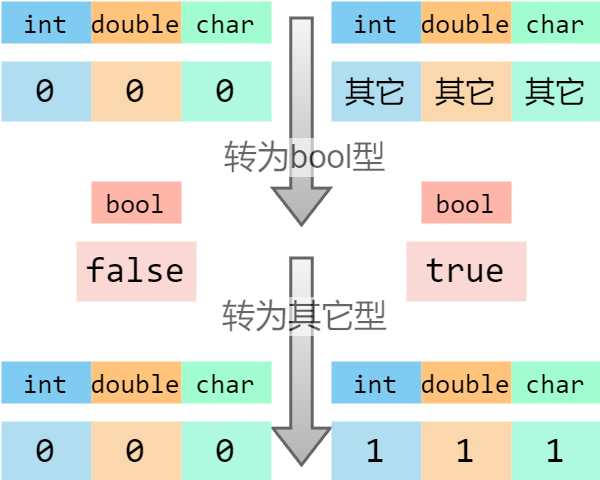
\includegraphics[width=0.7\textwidth]{../images/generalized_parts/02_boolean_conversion.png}
    \caption{布尔转换规则}
\end{figure}
\subsection*{显式类型转换}
隐式类型转换固然方便,但并不是任何时候都能满足我们的需要;有些时候甚至会背离我们的需要,从而造成很多不便。对于这种情况,\textbf{显式类型转换(Explicit type conversion)}就比较有用了。\par
C风格的显式类型转换语法是
\begin{lstlisting}
    (<类型>) <数据>
\end{lstlisting}
这样就能得到目标类型的一个临时变量,我们可以拿它去计算了。\par
比如说,如果我要把整数运算 \lstinline@a/b@ 变为浮点运算,那么我可以这样写:
\begin{lstlisting}
    cout << (double) a / (double) b; //显式类型转换
\end{lstlisting}
实际上我们只要写一个显式类型转换就可以了,另一个操作数自然会被隐式类型转换过去,不用麻烦我们再写一遍了。\par
如果我们嫌弃 \lstinline@double@ 类型的精度不够高,解决方法就是显式地转换为 \lstinline@long double@ 类型!
\begin{lstlisting}
    cout << (long double) a / b; //显式类型转换;b会被隐式转换为long double
\end{lstlisting}\par
在C++中,模运算不支持浮点型到整型的隐式类型转换,比如本节开头的例子里就体现了这一点。在保证两个操作数为整数的前提下(实际上不是整数也可以,不过两个小数本来就不可以取模,强行取模又有什么意思呢),我们也可以使用显式类型转换。\par
C++中引入了两类新的显式类型转换风格:一类是构造函数风格的类型转换;另一类是包含 \lstinline@static_cast@ 在内的四种特定类型转换语法。构造函数风格的类型转换语法为
\begin{lstlisting}
    <类型> (<数据>)
\end{lstlisting}
比如说上述的除法可以写作 \lstinline@double(a)/double(b)@\footnote{注意:它不适合类型关键字中间有空格的类型,比如 \lstinline@unsigned char@ 和 \lstinline@long  double@。}。而四种特定类型转换语法中我们只讲\\\lstinline@static_cast@,其余的留到精讲篇。它的语法是
\begin{lstlisting}
    static_cast<[类型]> ([数据])
\end{lstlisting}
在这里我为了避开括号对 \lstinline@<>@,转而使用括号对 \lstinline@[]@ 来表达,请读者留意。\par
C风格类型转换(和构造函数风格类型转换)最大的好处就是方便。它是一种比较``粗暴''的类型转换方式\footnote{它是 \lstinline@const_cast@, \lstinline@static_cast@ 和 \lstinline@reinterpret_cast@ 三种转换方法的统合体。},写起来又很简单,所以新手程序员更青睐这种写法。但是在面对复杂类型转换,尤其是涉及指针等复合类型的时候,这样的转换很容易出错。因而,出于类型安全的考量,指定类型转换方式要更稳妥些。我也建议读者按照自己的需求,尽量使用 \lstinline@static_cast@ 等特定的转换语法,避免C风格那种大包大揽的转换。\par
比如说,如果我们要用 \lstinline@static_cast@ 来实现 \lstinline@double@ 型转 \lstinline@int@ 型并进行取模运算,我们可以这样写:
\begin{lstlisting}
    cout << static_cast<int> (a) % static_cast<int> (b);
    //将a和b都类型转换为int,然后就可以使用模运算了
\end{lstlisting}
这里需要多加注意,无论你使用哪种风格的类型转换语法,在这里必须将 \lstinline@a@ 和 \lstinline@b@ 都显式类型转换为 \lstinline@int@,因为在模运算中没有整数和浮点数之间的隐式类型转换规则。\par
而假如你想要把 \lstinline@double@ 型转换为 \lstinline@int@ 型来进行四则运算的话,你就要注意把每个数据都转化成 \lstinline@int@ 型,不然……
\begin{lstlisting}
    double a, b; //定义浮点变量a,b
    cin >> a >> b; //输入a和b
    cout << static_cast<int> (a) * b; //试图进行显式类型转换
\end{lstlisting}
在这里,乘法运算符在面临一个 \lstinline@int@ 操作数和 \lstinline@double@ 操作数的时候,它会怎么做呢?如图2.5所示,它将把 \lstinline@int@ 通过隐式类型转换变为 \lstinline@double@ 型!这样一来我们就白干了。\par
\begin{figure}[htbp]
    \centering
    \includegraphics[width=0.6\textwidth]{../images/generalized_parts/02_Explicit_type_cast_from_double_to_int_in_vain.png}
    \caption{显式类型转换,但是又被隐式类型转换改回去了}
\end{figure}
总而言之,类型转换是一个非常复杂的话题。限于我们目前接触到的类型尚少,这里只作简单概括。将来我们接触复合类型和自定义类型的时候,还会对此作针对性讲解的。\par
